\documentclass[a4paper,14pt]{extarticle}

\usepackage[a4paper,top=20mm,bottom=20mm,left=30mm,right=10mm]{geometry}
\usepackage[T1,T2A]{fontenc}
\usepackage[utf8]{inputenc}
\usepackage[russian]{babel}
\usepackage{indentfirst}
\usepackage{titlesec}
\usepackage{graphicx}
\usepackage{verbatim}
\usepackage{fancyvrb}

\renewcommand{\baselinestretch}{1.3}
\setlength{\parindent}{12.5mm}
\titleformat{\section}{\normalsize\bfseries}{\indent\thesection}{1em}{}
\titleformat{\subsection}{\normalsize\bfseries}{\indent\thesubsection}{1em}{}

\begin{document}

  \newpage\thispagestyle{empty}
  \begin{center}
    \MakeUppercase{
      Министерство науки и высшего образования Российской Федерации\\
      Федеральное государственное бюджетное образовательное учреждение высшего образования\\
      <<Вятский Государственный Университет>>\\
    }
    Институт математики и информационных систем\\
    Факультет автоматики и вычислительной техники\\
    Кафедра электронных вычислительных машин
  \end{center}
  \vfill

  \begin{center}
    \textbf{Поиск путей в графах}\\
    Отчёт по лабораторной работе №6\\
    по дисциплине\\
    <<Дискретная математика>>\\
    Вариант 6
  \end{center}
  \vfill

  \noindent
  \begin{tabular}{ll}
    Выполнил студент гр. ИВТб-1301-05-00 \hspace{5mm} &
    \rule[-1mm]{25mm}{0.10mm}\,/Макаров С.А./\\
    
    Руководитель преподаватель & \rule[-1mm]{25mm}{0.10mm}\,/Пахарева И.В./\\
  \end{tabular}

  \vfill
  \begin{center}
    Киров 2025
  \end{center}

  \newpage
  \section*{\hspace{12.5mm}Цель}
  Цель лабораторной работы: изучение основ теории графов, поиск элементарных путей, разработка приложения на языке Паскаль или СИ согласно заданию.

  \section*{\hspace{12.5mm}Задание}
  Орграф задан матрицей смежности в файле (вершин >= 5, дуг >= 5). Найти возможные элементарные пути (вершины в пути не повторяются) из вершины, имя которой вводится с клавиатуры.

  \section*{\hspace{12.5mm}Решение}

  Для решения задач подготовлен ориентированный граф, представленный на рисунке 1.

  \begin{figure}[h]
    \centering
    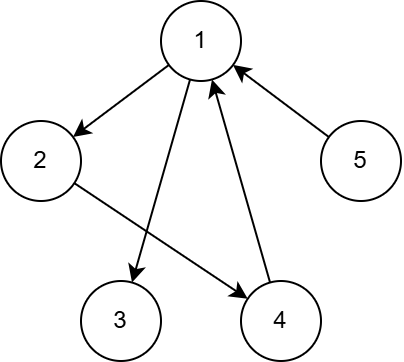
\includegraphics[width=0.4\linewidth]{images/graph.png}
  \end{figure}
  \begin{center}
    Рисунок 1 – Ориентированный граф
  \end{center}

  \pagebreak

  \pagebreak
  При разработке реализована программа, исходный код которой представлен ниже.

  \begingroup
    \linespread{1}

    \begin{Verbatim}[tabsize=2]
{$codepage UTF8}

uses
  SysUtils;

const
  MAX_SIZE = 5;

type
  TMatrix = array[1..MAX_SIZE, 1..MAX_SIZE] of integer;
  TVisited = array[1..MAX_SIZE] of boolean;
  TPath = array[1..MAX_SIZE] of integer;

var
  adjacency: TMatrix;
  visited: TVisited;
  path: TPath;
  startVertex: integer;

procedure ReadMatrix(var matrix: TMatrix);
var
  fileInput: text;
  fileLine: string;
  i, j, k: integer;
begin
  Assign(fileInput, 'input.txt');
  Reset(fileInput);

  i := 1;
  while not Eof(fileInput) do
  begin
    Readln(fileInput, fileLine);

    j := 1;
    for k := 1 to Length(fileLine) do
    begin
      if fileLine[k] <> ' ' then
      begin
        matrix[i, j] := StrToInt(fileLine[k]);
        j := j + 1;
      end;
    end;
    i := i + 1;
  end;

  Close(fileInput);
end;

procedure PrintMatrix(var matrix: TMatrix);
var
  i, j: integer;
begin
  Write('  ');
  for i := 1 to MAX_SIZE do
    Write(' ', i, ' ');
  Writeln();

  for i := 1 to MAX_SIZE do
  begin
    Write(i, '  ');
    for j := 1 to MAX_SIZE do
      Write(matrix[i, j], '  ');
    Writeln();
  end;
end;

procedure PrintPath(pathLength: integer);
var
  i: integer;
begin
  for i := 1 to pathLength - 1 do
    Write(path[i], ' -> ');
  Writeln(path[pathLength]);
end;

procedure DFS(current, target, pathLength: integer);
var
  i: integer;
begin
  visited[current] := true;
  path[pathLength] := current;

  if current <> target then
  begin
    for i := 1 to MAX_SIZE do
      if (adjacency[current, i] <> 0) and not visited[i] then
        DFS(i, target, pathLength + 1);
  end
  else
    PrintPath(pathLength);

  visited[current] := false;
end;

procedure FindAllPaths(startVertex: integer);
var
  i: integer;
begin
  for i := 1 to MAX_SIZE do
    visited[i] := false;

  for i := 1 to MAX_SIZE do
    if i <> startVertex then
      DFS(startVertex, i, 1);
end;

begin

  ReadMatrix(adjacency);
  Writeln(#10, 'Матрица смежности', #10);
  PrintMatrix(adjacency);

  Write(#10, 'Введите начальную вершину: ');
  Readln(startVertex);

  Writeln('Список всех элементарных путей');
  FindAllPaths(startVertex);

  Readln;

end.
    \end{Verbatim}
  \endgroup

  \pagebreak
  Экранная форма программы в виде консольного приложения представлена на рисунке 8.

  \begin{figure}[h]
    \centering
    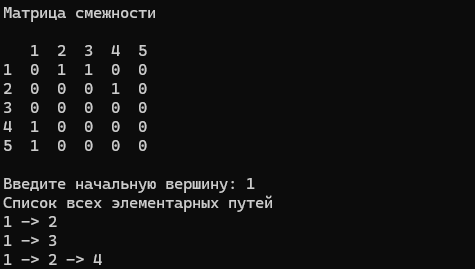
\includegraphics[width=0.8\linewidth]{images/image.png}
  \end{figure}
  \begin{center}
    Рисунок 8 – Консольный интерфейс программы
  \end{center}

  \section*{\hspace{12.5mm}Вывод}
  В процессе выполнения лабораторной работы, при решении предложенных задач, реализована программа на языке Паскаль, которая находит возможные элементарные пути из вершины согласно матрице смежности.

\end{document}